\graphicspath{{./1-Proyecto/capitulo2/}}

\chapter{Archimate}{
    \section{Introducción}
    En el contexto de la Arquitectura Empresarial, contar con un lenguaje de modelado estandarizado resulta esencial para representar de manera clara y coherente los diferentes dominios organizacionales. En este sentido, Archimate surge como una solución práctica y ampliamente adoptada que permite modelar, describir, analizar y comunicar arquitecturas complejas de forma estructurada.

    ArchiMate es un lenguaje de modelado abierto, desarrollado y respaldado por The Open Group, que proporciona una notación visual unificada para representar las relaciones entre procesos de negocio, aplicaciones y tecnología. Su objetivo es facilitar la comprensión de la arquitectura empresarial tanto para los equipos técnicos como para los diferentes grupos de interés de una organización, permitiendo una visión integral y coherente del estado actual y futuro de la empresa.

    Gracias a su enfoque estructurado, Archimate permite visualizar cómo los cambios en un área afectan a otras, promoviendo la alineación estratégica entre el negocio y las tecnologías de la información. Asimismo, ofrece una base sólida para el análisis de impacto, la toma de decisiones y la gestión de transformaciones organizacionales.

    Este capítulo explora las bases conceptuales de Archimate, sus principales características, y su papel como lenguaje complementario dentro del desarrollo de la arquitectura empresarial con TOGAF.
	\section{¿Qué es Archimate?}
    \textbf{ArchiMate es un lenguaje de modelado de arquitectura empresarial} abierto e independiente para respaldar la descripción, el análisis y la visualización de la arquitectura dentro y entre dominios comerciales de manera inequívoca.\\\
    ArchiMate ofrece un lenguaje común para describir la construcción y operación de procesos comerciales, estructuras organizativas, flujos de información, sistemas de TI e infraestructura técnica. Esta información ayuda a las partes interesadas a diseñar, evaluar y comunicar las consecuencias de las decisiones y los cambios dentro y entre estos dominios comerciales. \cite{Archimate_definition}
	\section{Características}	
	ArchiMate es un  estándar abierto  mantenido y actualizado por The Open Group. Se tienen en cuenta los últimos desarrollos e ideas en arquitectura empresarial y el marco ArchiMate se mejora continuamente. Algunas de las características que posee Archimate son:
    \begin{itemize}
        \item ArchiMate garantiza la coherencia en todos los modelos de arquitectura, por lo que es un lenguaje ágil y sencillo. 
        \item Contiene suficientes conceptos para modelar la arquitectura empresarial y no incluye todos los conceptos posibles para no salirse de sus propios límites. Como resultado, la arquitectura empresarial se puede comunicar de manera clara y coherente en todos los dominios de su negocio. 
        \item Su estructura uniforme hace que sea fácil de aprender y aplicar.
        \item ArchiMate permite realizar un modelado de alto nivel dentro de un dominio, es también bases para el análisis de identificación de procesos, actores, entre otros elementos involucrados en una arquitectura empresarial, este lenguaje se ofrece así como un complemento que ofrece metodologías que permiten desarrollar una arquitectura empresarial.
        \item ArchiMate ofrece una forma de generalización de comunicación a nivel empresarial, lo que potencializa la velocidad con la cual se puede conocer un proceso o elemento que pertenece a una arquitectura empresarial.
    \end{itemize}
    
    %---------------------- CAPA DE RELACIONES ------------------------%
    \section{Capas}
	%--------------------------------------------CAPA DE RELACIONES------------------------------------------------------%

\subsection{Relaciones y conectores de relaciones}
% Descripción introductoria de las relaciones en ArchiMate
El lenguaje ArchiMate define un conjunto central de relaciones genéricas, cada una de las cuales puede conectar un conjunto predefinido de conceptos de origen y destino (en la mayoría de los casos, elementos, pero en algunos casos también otras relaciones). Muchas de estas relaciones están “sobrecargadas”; es decir, su significado exacto difiere según los conceptos de origen y destino que conectan. Las Tablas \ref{tab:Tabla de relaciones 1}, \ref{tab:Tabla de relaciones 2} y \ref{tab:Tabla de relaciones 3} ofrecen una descripción general de las relaciones de ArchiMate con sus definiciones. \cite{archimate} 

%---------------------------------------------------------------------------------------------------------
% TABLA 1: RELACIONES ESTRUCTURALES
%---------------------------------------------------------------------------------------------------------
\begin{longtable}{|p{0.15\linewidth}|p{0.45\linewidth}|p{0.2\linewidth}|p{0.2\linewidth}|}
    % Configuración de la caption y encabezado
    \caption{Tabla de relaciones estructurales} \label{tab:Tabla de relaciones 1} \\
    \hline
    \rowcolor[HTML]{DAE8FC} 
    \textbf{Relaciones estructurales} & \textbf{Definición} & \textbf{Notación} & \textbf{Nombres de Roles} \\
    \hline
    \endhead % Fin del encabezado repetido en cada página
    \hline
    \multicolumn{4}{r}{\textit{Continúa en la siguiente página}} \\
    \endfoot % Pie de página en páginas intermedias
    \hline
    \endlastfoot % Fin de la tabla en la última página

    % Fila 1: Composición
    Composición &
    Representa que un elemento consta de uno o más conceptos. &
    \begin{center}
        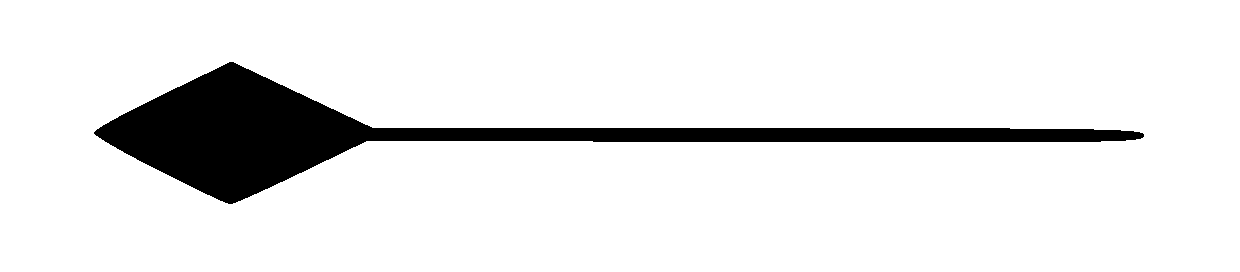
\includegraphics[width=1\linewidth]{imgs/relaciones/composicion.pdf}
    \end{center} &
    \begin{center}
        → compuesto de \\ ← compuesto en
    \end{center} \\
    \hline

    % Fila 2: Agregación
    Agregación &
    Representa que un elemento combina uno o más conceptos. &
    \begin{center}
        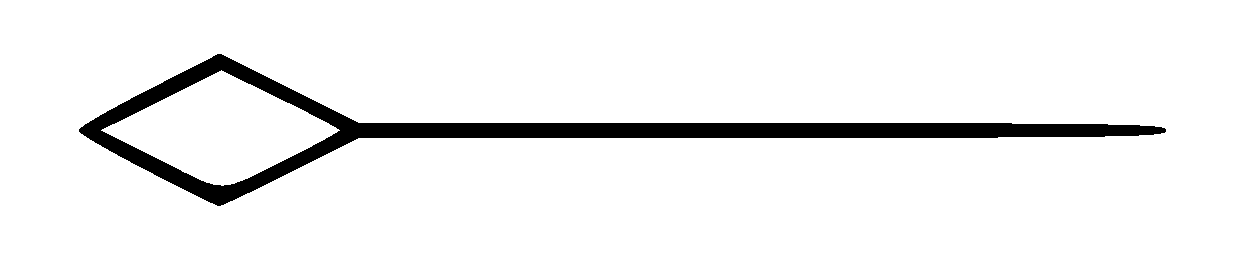
\includegraphics[width=1\linewidth]{imgs/relaciones/agregacion.pdf}
    \end{center} &
    \begin{center}
        → agregados \\ ← agregado en
    \end{center} \\
    \hline

    % Fila 3: Asignación
    Asignación &
    Representa la asignación de responsabilidad, desempeño de comportamiento, almacenamiento o ejecución. &
    \begin{center}
        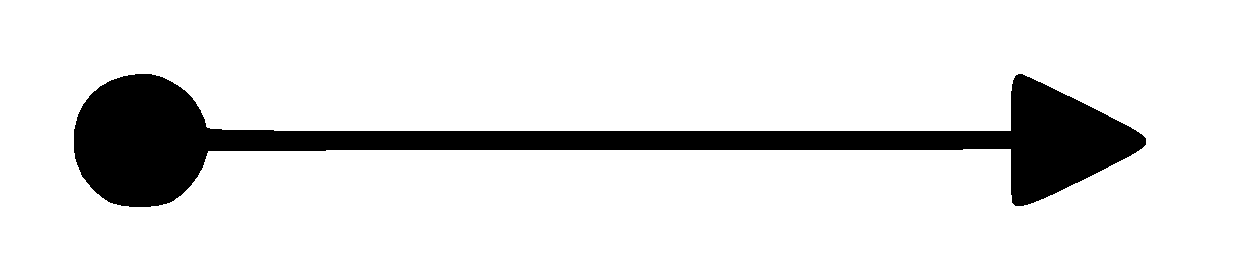
\includegraphics[width=1\linewidth]{imgs/relaciones/asignacion.pdf}
    \end{center} &
    \begin{center}
        → asignado a \\ ← ha asignado
    \end{center} \\
    \hline

    % Fila 4: Realización
    Realización &
    Representa que un elemento juega un papel crítico en la creación, logro, sustento u operación de un elemento más abstracto. &
    \begin{center}
        
\includegraphics[width=1\linewidth]{imgs/relaciones/realizacion.pdf}
    \end{center} &
    \begin{center}
        → realiza \\ ← realizado por
    \end{center} \\
    \hline
\end{longtable}

%---------------------------------------------------------------------------------------------------------
% TABLA 2: RELACIONES DE DEPENDENCIA
%---------------------------------------------------------------------------------------------------------
\begin{longtable}{|p{0.15\linewidth}|p{0.45\linewidth}|p{0.2\linewidth}|p{0.2\linewidth}|}
    % Configuración de la caption y encabezado
    \caption{Tabla de relaciones de dependencia} \label{tab:Tabla de relaciones 2} \\
    \hline
    \rowcolor[HTML]{DAE8FC} 
    \textbf{Relaciones de dependencia} & \textbf{Definición} & \textbf{Notación} & \textbf{Nombres de Roles} \\
    \hline
    \endhead % Fin del encabezado repetido en cada página
    \hline
    \multicolumn{4}{r}{\textit{Continúa en la siguiente página}} \\
    \endfoot % Pie de página en páginas intermedias
    \hline
    \endlastfoot % Fin de la tabla en la última página

    % Fila 1: Servicio
    Servicio &
    Representa que un elemento proporciona su funcionalidad a otro elemento. &
    \begin{center}
        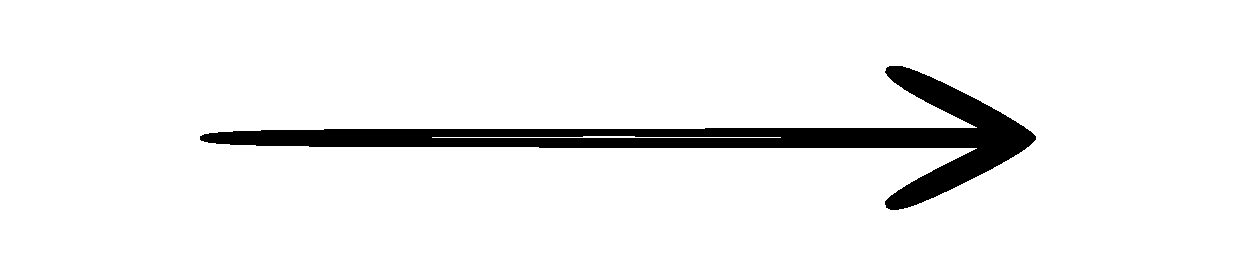
\includegraphics[width=1\linewidth]{imgs/relaciones/servicio.pdf}
    \end{center} &
    \begin{center}
        → sirve \\ ← servido por
    \end{center} \\
    \hline

    % Fila 2: Acceso
    Acceso &
    Representa la capacidad del comportamiento y de los elementos de la estructura activa para observar o actuar sobre los elementos de la estructura pasiva. &
    \begin{center}
        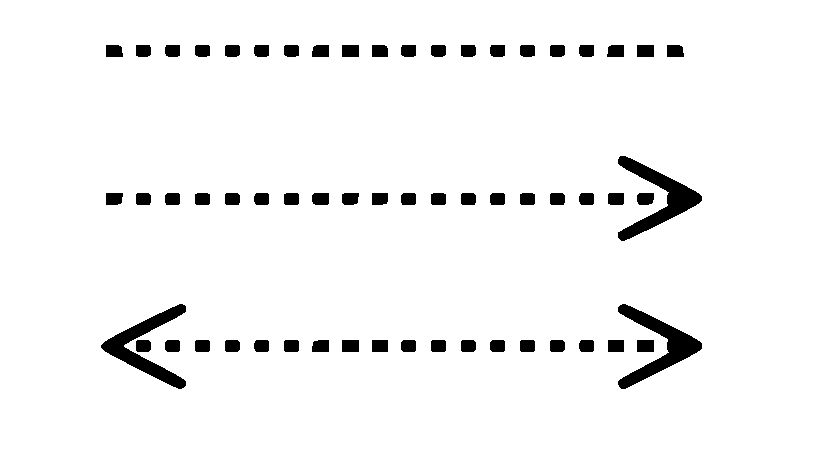
\includegraphics[width=1\linewidth]{imgs/relaciones/acceso.pdf}
    \end{center} &
    \begin{center}
        → accesos \\ ← accedido por
    \end{center} \\
    \hline

    % Fila 3: Influencia
    Influencia &
    Representa que un elemento afecta la implementación o logro de algún elemento de motivación. &
    \begin{center}
        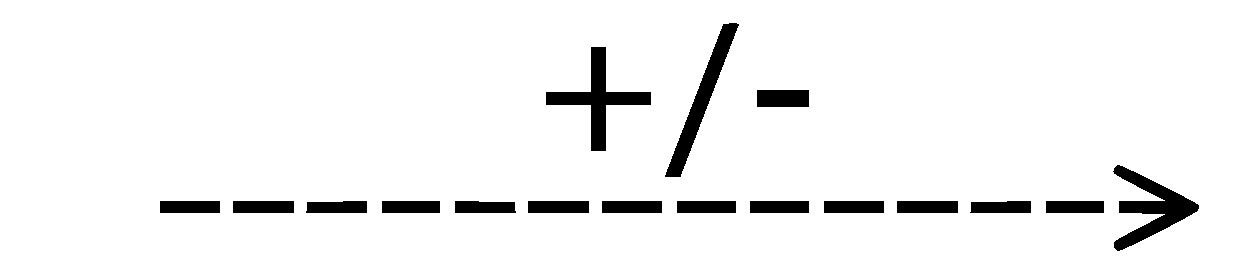
\includegraphics[width=1\linewidth]{imgs/relaciones/influencia.pdf}
    \end{center} &
    \begin{center}
        → influye \\ ← influido por % Corrección semántica para consistencia
    \end{center} \\
    \hline

    % Fila 4: Asociación
    Asociación &
    Representa una relación no especificada o una que no está representada por otra relación ArchiMate. &
    \begin{center}
        
\includegraphics[width=1\linewidth]{imgs/relaciones/asociacion.pdf}
    \end{center} &
    \begin{center}
        → asociado a \\ ← asociado de
    \end{center} \\
    \hline
\end{longtable}

%---------------------------------------------------------------------------------------------------------
% TABLA 3: CONECTORES DE RELACIONES
%---------------------------------------------------------------------------------------------------------
\begin{longtable}{|p{0.15\linewidth}|p{0.45\linewidth}|p{0.2\linewidth}|p{0.2\linewidth}|}
    % Configuración de la caption y encabezado
    \caption{Tabla de conectores de relaciones} \label{tab:Tabla de relaciones 3} \\
    \hline
    \rowcolor[HTML]{DAE8FC} 
    \textbf{Conectores de relación} & \textbf{Definición} & \textbf{Notación} & \textbf{Nombres de Roles} \\
    \hline
    \endhead % Fin del encabezado repetido en cada página
    \hline
    \multicolumn{4}{r}{\textit{Continúa en la siguiente página}} \\
    \endfoot % Pie de página en páginas intermedias
    \hline
    \endlastfoot % Fin de la tabla en la última página

    % Fila 1: Unión
    Unión &
    Se utiliza para conectar relaciones del mismo tipo. &
    \begin{center}
        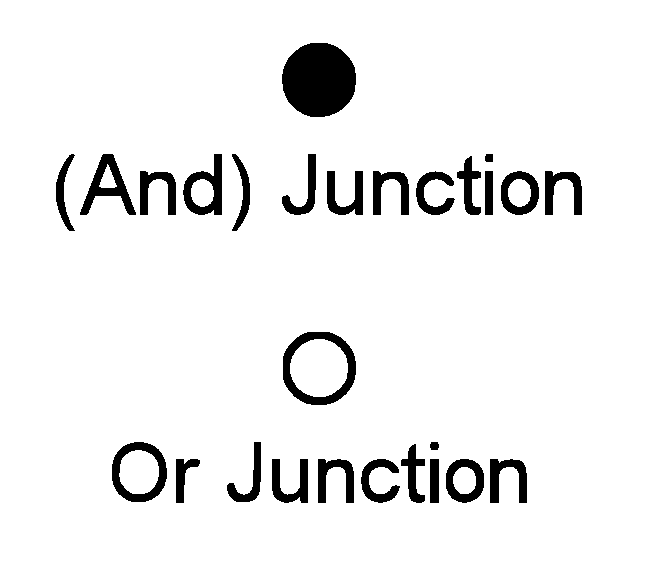
\includegraphics[width=1\linewidth]{imgs/relaciones/union.pdf}
    \end{center} &
    \begin{center}
        → asociado a \\ ← asociado de
    \end{center} \\
    \hline
\end{longtable}
	%--------------------------------------------CAPA MOTIACIONAL ------------------------------------------------------%


\subsection{Capa motivacional}

Los elementos de motivación se utilizan para modelar las motivaciones o \textbf{razones que guían el diseño o cambio de una arquitectura empresarial.}

La tabla \ref{tab:Tabla de la capa de motivación} ofrece una visión general de los elementos de motivación, con sus definiciones. \cite{archimate}

\begin{longtable}{|p{0.15\linewidth}|p{0.45\linewidth}|p{0.2\linewidth} p{0.2\linewidth}|}
    \caption{Tabla de la capa de motivación}
    \\
    \hline
    \rowcolor[HTML]{DAE8FC} 
    \textbf{Elemento} & \textbf{Definición} & \multicolumn{2}{c|}{\textbf{Notación}} \\
    \hline
    \endhead
    \hline
    \multicolumn{4}{r}{\textit{Continúa en la siguiente página}} \\
    \endfoot
    \hline
    \endlastfoot
    \label{tab:Tabla de la capa de motivación}
    %Contenido 1 &
    %\lipsum[1] &
    %Datos A1
    %& Datos B1
    %\\
    %\hline

    Interesado &
    Representa el papel de un individuo, equipo u organización (o clases de ellos) que representa sus intereses en los efectos de la arquitectura. &
\begin{center}
    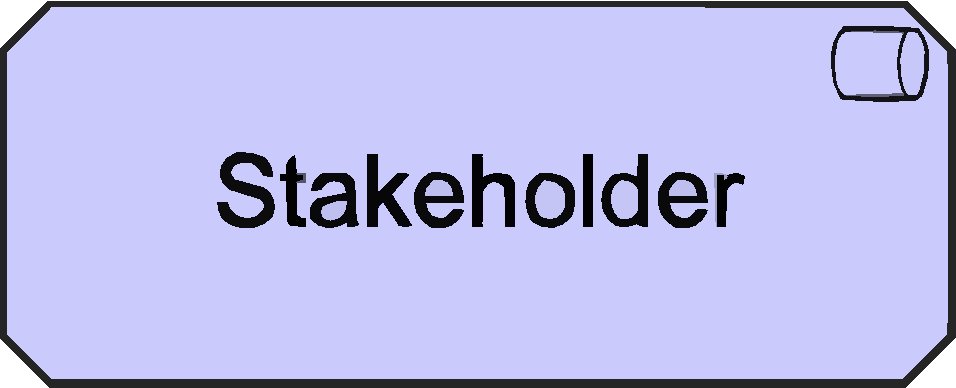
\includegraphics[width=1\linewidth]{imgs/capa_motivacional/stakeholder1.pdf}
\end{center} &
\begin{center}
    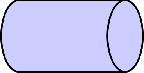
\includegraphics[width=0.7\linewidth]{imgs/capa_motivacional/stakeholder2.pdf}
\end{center}
    \\ \hline

    Conductor &
    Representa una condición externa o interna que motiva a una organización a definir sus objetivos e implementar los cambios necesarios para alcanzarlos. &
\begin{center}
    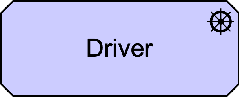
\includegraphics[width=1\linewidth]{imgs/capa_motivacional/driver1.pdf}
\end{center} &
\begin{center}
    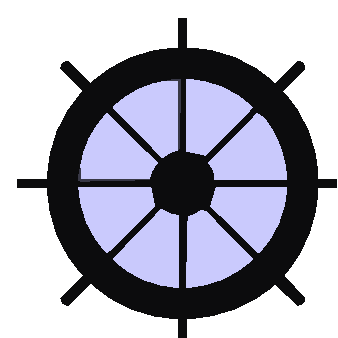
\includegraphics[width=0.5\linewidth]{imgs/capa_motivacional/driver2.pdf}
\end{center}
    \\ \hline

    Evaluación &
    Representa el resultado de un análisis del estado de cosas de la empresa con respecto a algún conductor. &
\begin{center}
    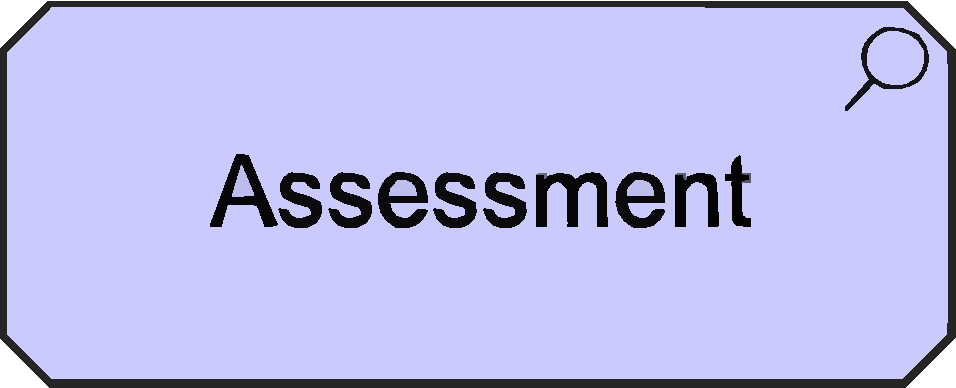
\includegraphics[width=1\linewidth]{imgs/capa_motivacional/assessment1.pdf}
\end{center} &
\begin{center}
    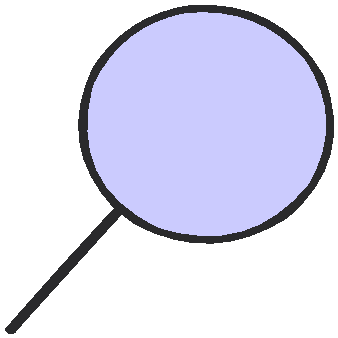
\includegraphics[width=0.5\linewidth]{imgs/capa_motivacional/assessment2.pdf}
\end{center}
    \\ \hline

    Meta &
    Representa una declaración de intención, dirección o estado final deseado de alto nivel para una organización y sus partes interesadas. &
\begin{center}
    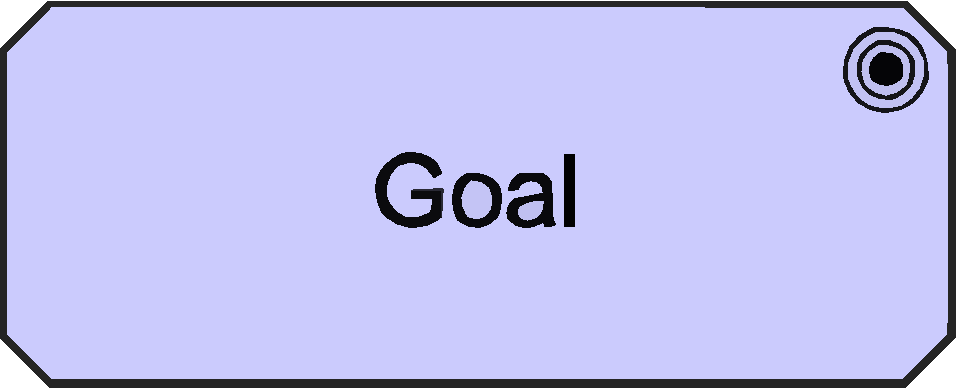
\includegraphics[width=1\linewidth]{imgs/capa_motivacional/goal1.pdf}
\end{center} &
\begin{center}
    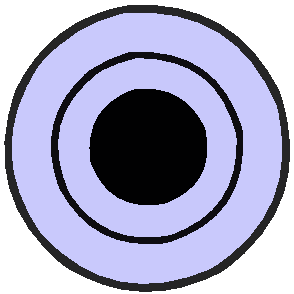
\includegraphics[width=0.5\linewidth]{imgs/capa_motivacional/goal2.pdf}
\end{center}
    \\ \hline

    Resultado &
    Representa un resultado final, efecto o consecuencia de un determinado estado de cosas. &
\begin{center}
    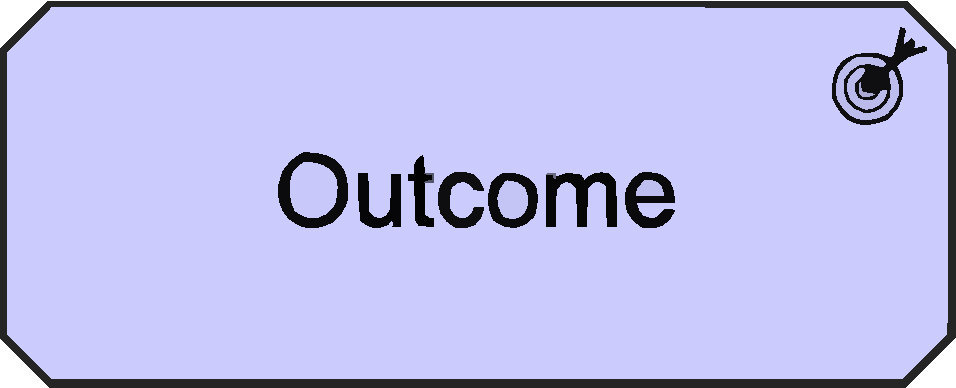
\includegraphics[width=1\linewidth]{imgs/capa_motivacional/outcome1.pdf}
\end{center} &
\begin{center}
    
\includegraphics[width=0.5\linewidth]{imgs/capa_motivacional/outcome2.pdf}
\end{center}
    \\ \hline

    Principio &
    Representa una declaración de intenciones que define una propiedad general que se aplica a cualquier sistema en un contexto determinado de la arquitectura. &
\begin{center}
    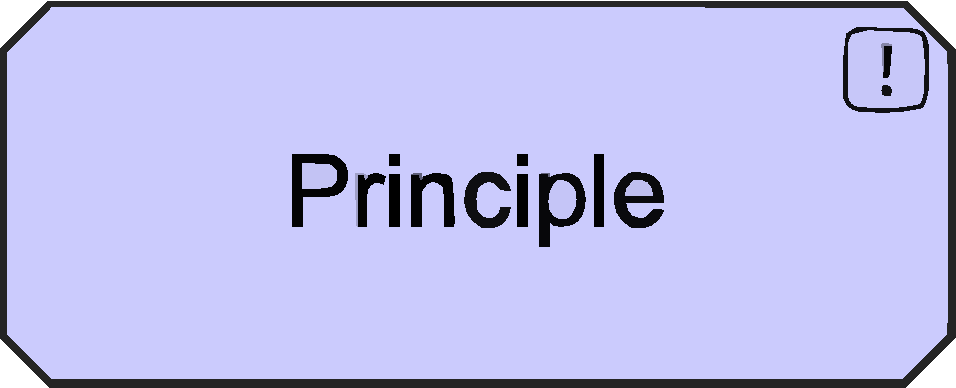
\includegraphics[width=1\linewidth]{imgs/capa_motivacional/principle1.pdf}
\end{center} &
\begin{center}
    
\includegraphics[width=0.5\linewidth]{imgs/capa_motivacional/principle2.pdf}
\end{center}
    \\ \hline

    Requisito &
    Representa una declaración de necesidad que define una propiedad que se aplica a un sistema específico según lo descrito por la arquitectura. &
\begin{center}
    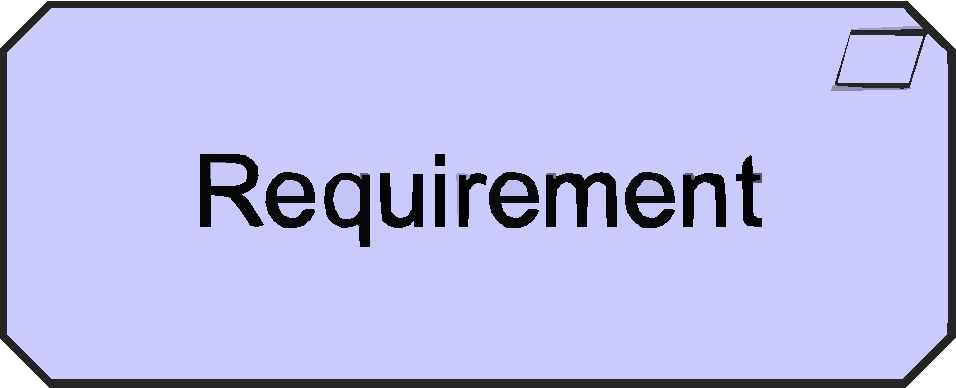
\includegraphics[width=1\linewidth]{imgs/capa_motivacional/requirement1.pdf}
\end{center} &
\begin{center}
    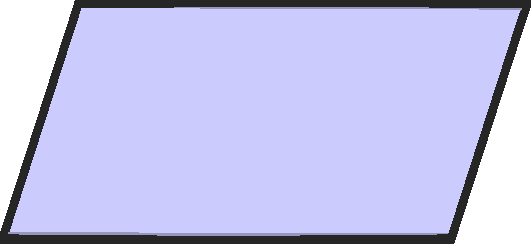
\includegraphics[width=0.5\linewidth]{imgs/capa_motivacional/requirement2.pdf}
\end{center}
    \\ \hline

    Restricción &
    Representa una limitación sobre aspectos de la arquitectura, su proceso de implementación o su realización. &
\begin{center}
    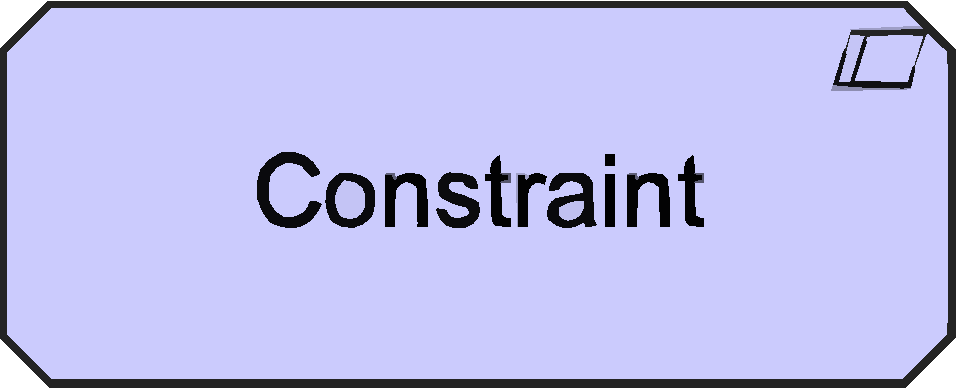
\includegraphics[width=1\linewidth]{imgs/capa_motivacional/constraint1.pdf}
\end{center} &
\begin{center}
    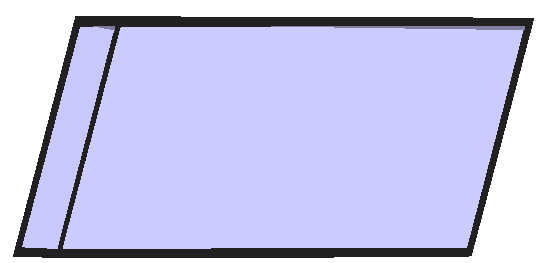
\includegraphics[width=0.5\linewidth]{imgs/capa_motivacional/constraint2.pdf}
\end{center}
    \\ \hline

    Significado &
    Representa el conocimiento o experiencia presente en, o la interpretación dada a, un concepto en un contexto particular. &
\begin{center}
    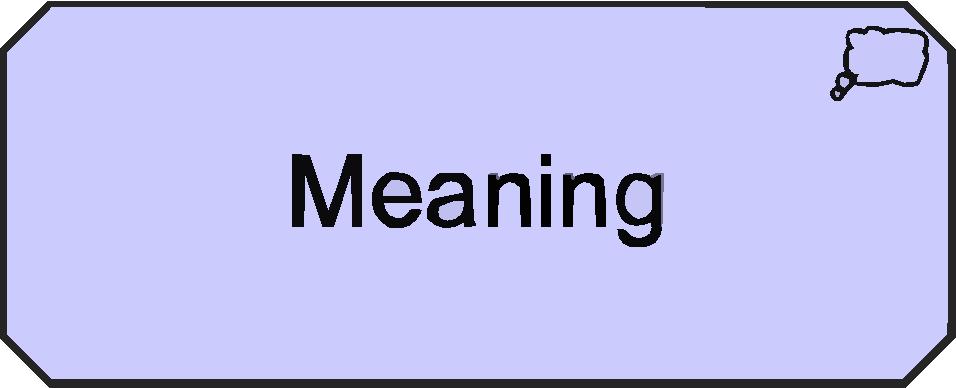
\includegraphics[width=1\linewidth]{imgs/capa_motivacional/meaning1.pdf}
\end{center} &
\begin{center}
    
\includegraphics[width=0.5\linewidth]{imgs/capa_motivacional/meaning2.pdf}
\end{center}
    \\ \hline

    Valor &
    Representa el valor relativo, la utilidad o la importancia de un concepto. &
\begin{center}
    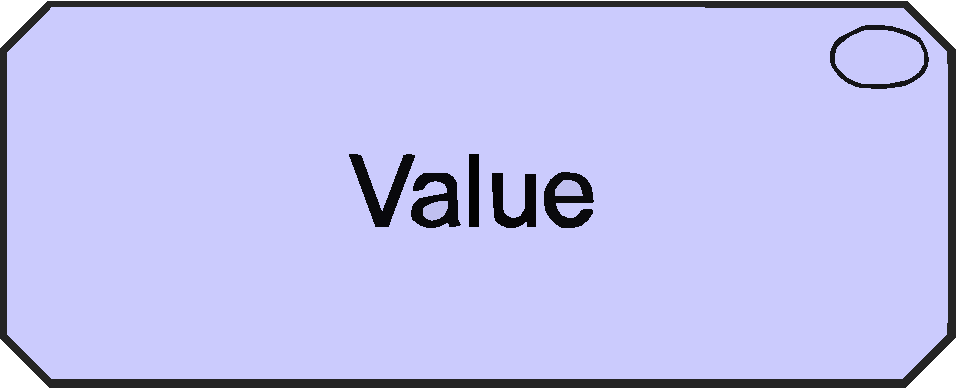
\includegraphics[width=1\linewidth]{imgs/capa_motivacional/value1.pdf}
\end{center} &
\begin{center}
    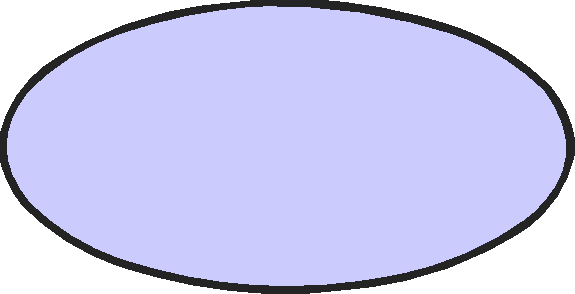
\includegraphics[width=0.5\linewidth]{imgs/capa_motivacional/value2.pdf}
\end{center}
    \\ \hline

\end{longtable}

	%--------------------------------------------CAPA DE ESTRATEGIAS ------------------------------------------------------%

\subsection{Capa de estrategias}
Los elementos de estrategia se utilizan normalmente para modelar la dirección estratégica y las opciones de una empresa, en lo que respecta al impacto en su arquitectura. Se pueden utilizar para expresar cómo la empresa quiere \textbf{crear valor para sus partes interesadas}, las capacidades que necesita, los recursos necesarios para respaldar estas capacidades, así como cómo planea configurar y utilizar estas capacidades y recursos para lograr sus objetivos. Los elementos de estrategia se utilizan para modelar la dirección estratégica y las opciones de la empresa, mientras que los elementos de la capa empresarial se utilizan para modelar la organización operativa de una empresa.

La tabla \ref{tab:Tabla de la capa de estrategia} ofrece una visión general de los elementos de la estrategia, con sus definiciones.\cite{archimate} 

\begin{longtable}{|p{0.15\linewidth}|p{0.45\linewidth}|p{0.2\linewidth} p{0.2\linewidth}|}
    \caption{Tabla de la capa de estrategia}
    \\
    \hline
    \rowcolor[HTML]{AFC5F6} 
    \textbf{Elemento} & \textbf{Descripción} & \multicolumn{2}{c|}{\textbf{Notación}} \\
    \hline
    \endhead
    \hline
    \multicolumn{4}{r}{\textit{Continúa en la siguiente página}} \\
    \endfoot
    \hline
    \endlastfoot
    \label{tab:Tabla de la capa de estrategia}
    %Contenido 1 &
    %\lipsum[1] &
    %Datos A1
    %& Datos B1
    %\\
    %\hline



    Recurso 
    &
    Representa un activo perteneciente o controlado por un individuo u organización. 
    &
\begin{center}
    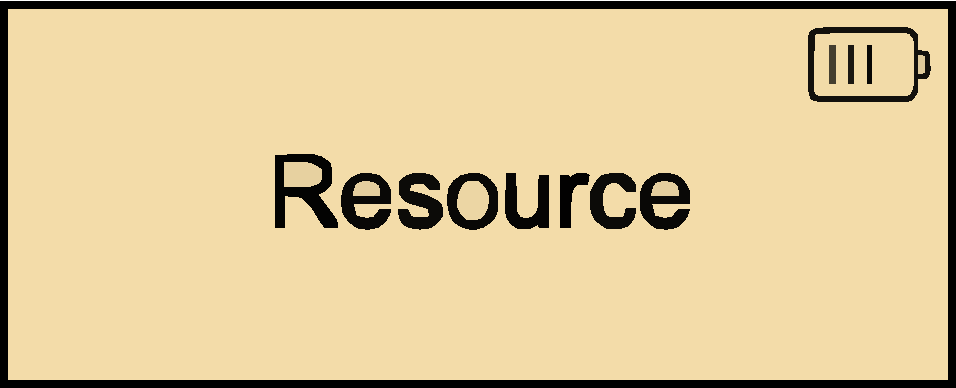
\includegraphics[width=1\linewidth]{imgs/capa_estrategia/fig-Resource-Notation_1.pdf}
\end{center} 
&
\begin{center}
    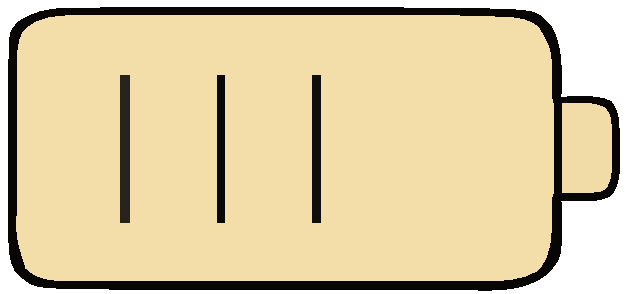
\includegraphics[width=0.8\linewidth]{imgs/capa_estrategia/fig-Resource-Notation_2.pdf}
\end{center}
    \\ \hline



    Capacidad 
    &
    Representa una condición externa o interna que motiva a una organización a definir sus objetivos e implementar los cambios necesarios para alcanzarlos. Representa una habilidad que un elemento activo de una estructura, como una organización, persona o sistema, posee. 
    &
\begin{center}
    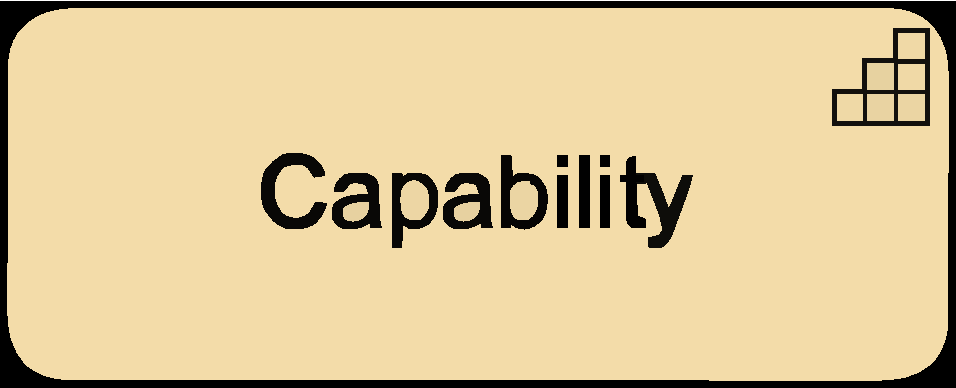
\includegraphics[width=1\linewidth]{imgs/capa_estrategia/fig-Capability-Notation_1.pdf}
\end{center} &
\begin{center}
    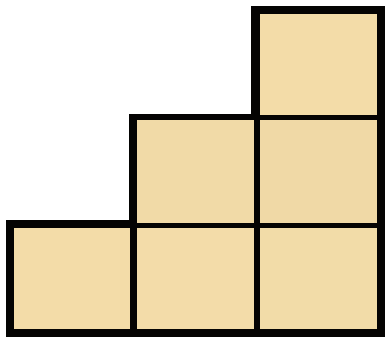
\includegraphics[width=0.5\linewidth]{imgs/capa_estrategia/fig-Capability-Notation_2.pdf}
\end{center}
    \\ \hline



    Transmisión de valor  
    &
    Representa una secuencia de actividades que generan un resultado general para un cliente, stakeholder o usuario final. 
    &
\begin{center}
    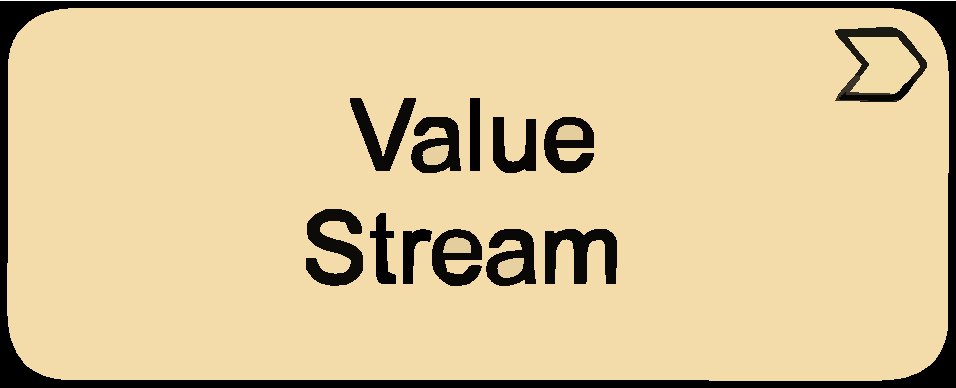
\includegraphics[width=1\linewidth]{imgs/capa_estrategia/fig-Value-Stream-Notation_1.pdf}
\end{center} &
\begin{center}
    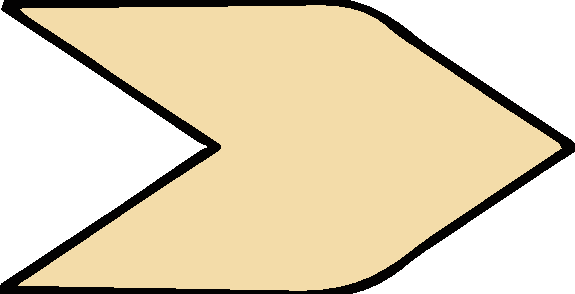
\includegraphics[width=0.5\linewidth]{imgs/capa_estrategia/fig-Value-Stream-Notation_2.pdf}
\end{center}
    \\ \hline



    Curso de acción 
    &
    Representa un acercamiento o plan para configurar algunas capacidades y recursos de la empresa, emprendidos para alcanzar una meta.
    &
\begin{center}
    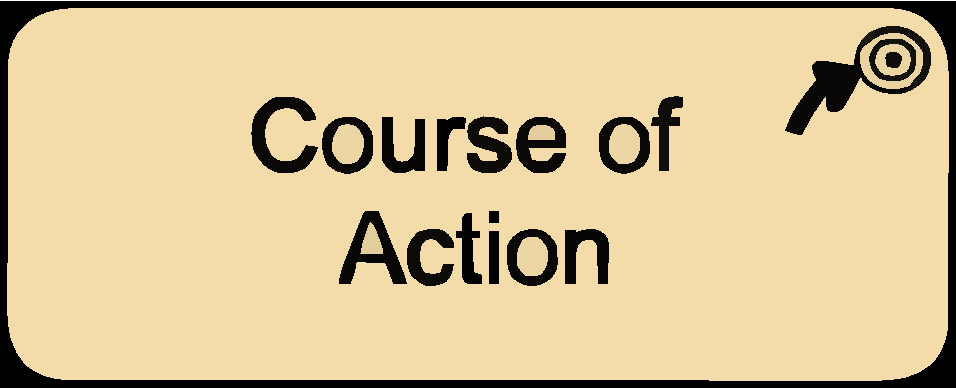
\includegraphics[width=1\linewidth]{imgs/capa_estrategia/fig-Course-of-Action-Notation_1.pdf}
\end{center} &
\begin{center}
    
\includegraphics[width=0.5\linewidth]{imgs/capa_estrategia/fig-Course-of-Action-Notation_2.pdf}
\end{center}
    \\ \hline


\end{longtable}
	%--------------------------------------------CAPA DE NEGOCIOS ------------------------------------------------------%

\subsection{Capa de negocios}
Los elementos de la capa empresarial se utilizan para modelar la \textbf{organización operativa} de una empresa de manera independiente de la tecnología, mientras que los elementos estratégicos se utilizan para modelar la dirección estratégica y las opciones de la empresa.

La tabla \ref{tab:Tabla de la capa de negocios} ofrece una descripción general de los elementos de la capa empresarial, con sus definiciones.\cite{archimate} 

\begin{longtable}{|p{0.15\linewidth}|p{0.45\linewidth}|p{0.2\linewidth} p{0.2\linewidth}|}
    \caption{Tabla de la capa de negocios}
    \\
    \hline
    \rowcolor[HTML]{AFC5F6} 
    \textbf{Elemento} & \textbf{Descripción} & \multicolumn{2}{c|}{\textbf{Notación}} \\
    \hline
    \endhead
    \hline
    \multicolumn{4}{r}{\textit{Continúa en la siguiente página}} \\
    \endfoot
    \hline
    \endlastfoot
    \label{tab:Tabla de la capa de negocios}
    %Contenido 1 &
    %\lipsum[1] &
    %Datos A1
    %& Datos B1
    %\\
    %\hline



    Actor comercial 
    &
    Representa una entidad comercial  que es capaz de realizar un comportamiento.
    &
\begin{center}
    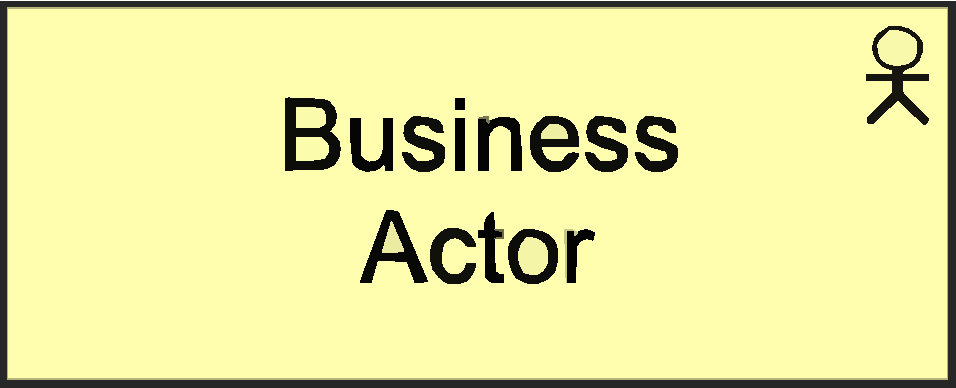
\includegraphics[width=1\linewidth]{imgs/capa_de_negocios/1.pdf}
\end{center} 
&
\begin{center}
    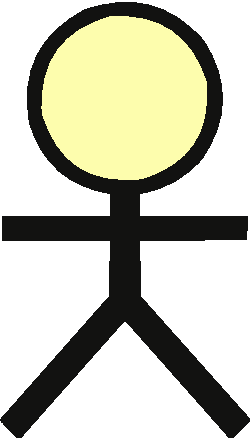
\includegraphics[width=0.3\linewidth]{imgs/capa_de_negocios/a1.pdf}
\end{center}
    \\ \hline



    Rol comercial 
    &
    Representa la responsabilidad de realizar un comportamiento específico, al que se puede asignar un actor, o el papel que juega un actor en una acción o evento particular.
    &
\begin{center}
    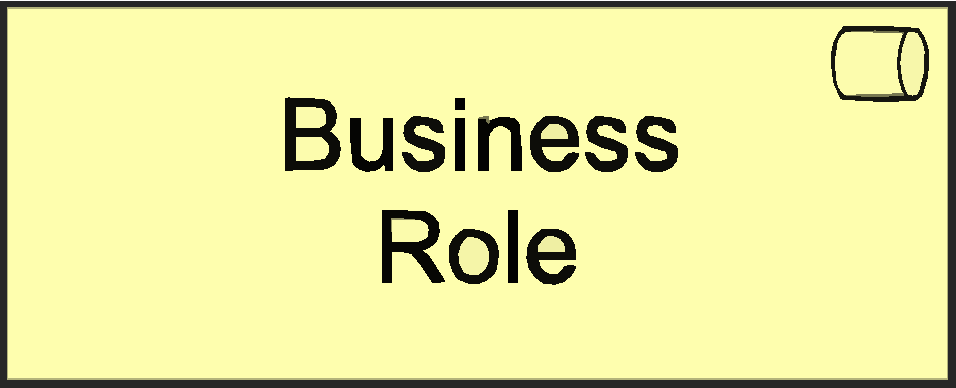
\includegraphics[width=1\linewidth]{imgs/capa_de_negocios/2.pdf}
\end{center} &
\begin{center}
    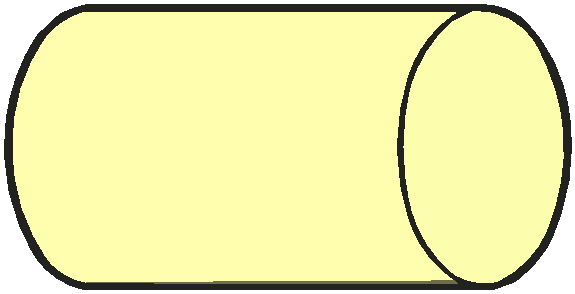
\includegraphics[width=0.5\linewidth]{imgs/capa_de_negocios/a2.pdf}
\end{center}
    \\ \hline



    Colaboración comercial
    &
    Representa un agregado de dos o más elementos de la estructura interna activa de la empresa que trabajan juntos para realizar un  comportamiento colectivo.
    &
\begin{center}
    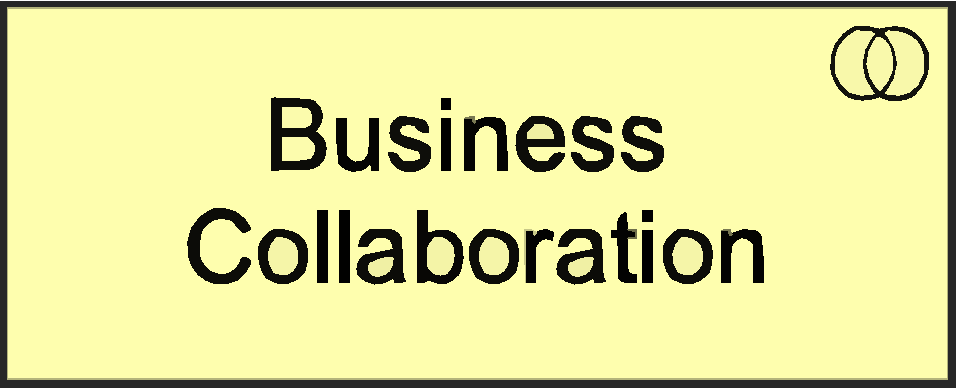
\includegraphics[width=1\linewidth]{imgs/capa_de_negocios/3.pdf}
\end{center} &
\begin{center}
    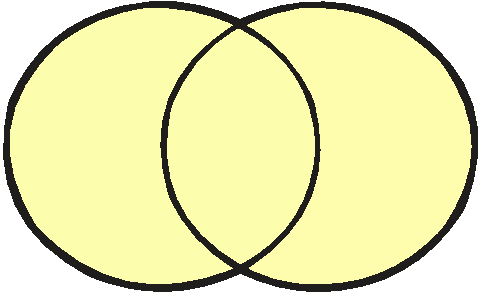
\includegraphics[width=0.5\linewidth]{imgs/capa_de_negocios/a3.pdf}
\end{center}
    \\ \hline



    Interfaz comercial
    &
    Representa un punto de acceso donde los servicios comerciales se ponen a disposición del entorno.
    &
\begin{center}
    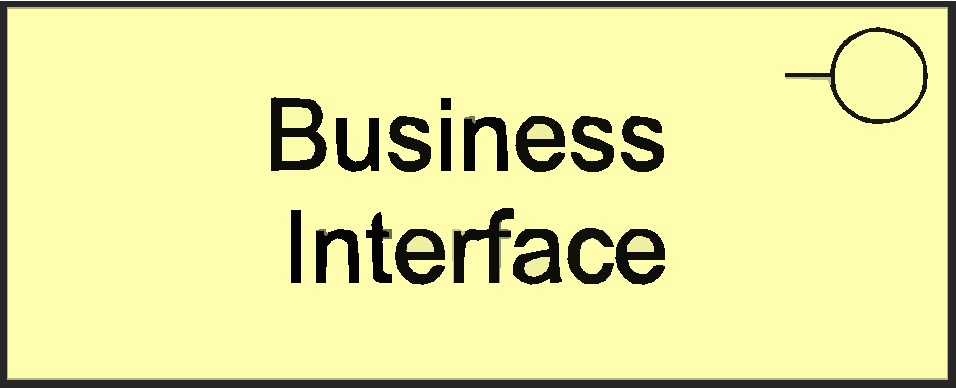
\includegraphics[width=1\linewidth]{imgs/capa_de_negocios/4.pdf}
\end{center} &
\begin{center}
    
\includegraphics[width=0.5\linewidth]{imgs/capa_de_negocios/a4.pdf}
\end{center}
    \\ \hline

    Proceso comercial
    &
    Representa una secuencia de comportamientos comerciales que logra un resultado específico, como un conjunto definido de productos o servicios comerciales.
    &
\begin{center}
    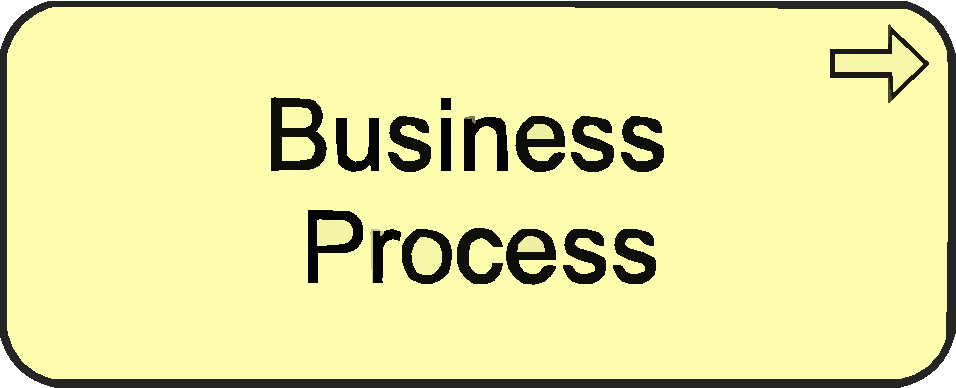
\includegraphics[width=1\linewidth]{imgs/capa_de_negocios/5.pdf}
\end{center} &
\begin{center}
    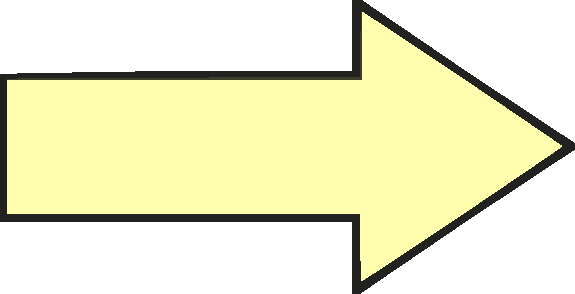
\includegraphics[width=0.5\linewidth]{imgs/capa_de_negocios/a5.pdf}
\end{center}
    \\ \hline


    Función comercial
    &
    Representa una colección de comportamiento comercial basado en un conjunto elegido de criterios, como los recursos comerciales necesarios y/o las competencias, y se gestiona o realiza como un todo.
    &
\begin{center}
    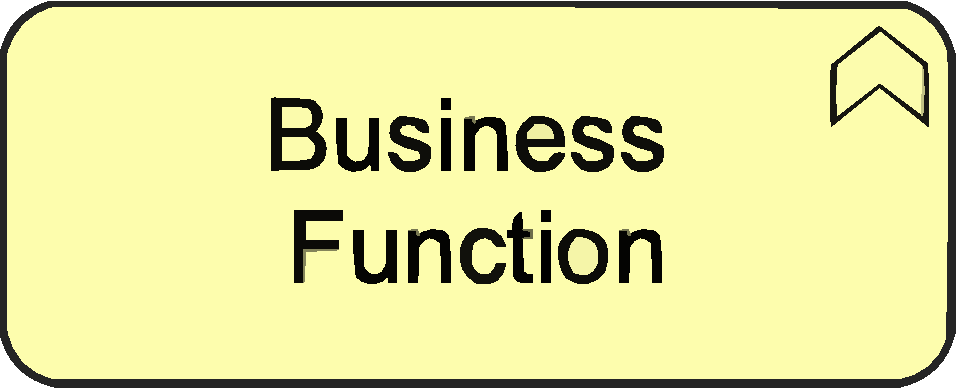
\includegraphics[width=1\linewidth]{imgs/capa_de_negocios/6.pdf}
\end{center} &
\begin{center}
    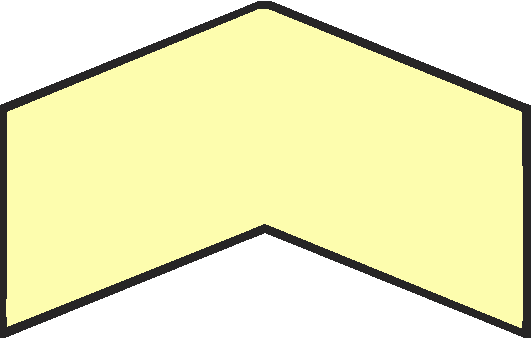
\includegraphics[width=0.5\linewidth]{imgs/capa_de_negocios/a6.pdf}
\end{center}
    \\ \hline

    Interacción comercial
    &
    Representa una unidad de comportamiento comercial colectivo realizado por (una  colaboración de) dos o más actores comerciales, roles comerciales o colaboraciones comerciales.
    &
\begin{center}
    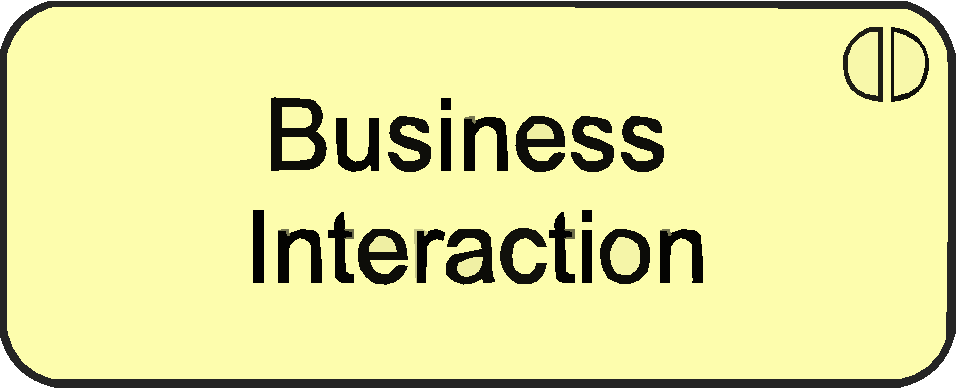
\includegraphics[width=1\linewidth]{imgs/capa_de_negocios/7.pdf}
\end{center} &
\begin{center}
    \includegraphics[width=0.5\linewidth]{imgs/capa_de_negocios/a7.pdf}
\end{center}
    \\ \hline


    Evento comercial
    &
    Representa un cambio de estado relacionado con el negocio.
    &
\begin{center}
    \includegraphics[width=1\linewidth]{imgs/capa_de_negocios/8.pdf}
\end{center} &
\begin{center}
    \includegraphics[width=0.5\linewidth]{imgs/capa_de_negocios/a8.pdf}
\end{center}
    \\ \hline

    Servicio comercial
    &
    Representa explícitamente el comportamiento definido que un rol comercial, un actor comercial o una colaboración comercial expone a su entorno.
    &
\begin{center}
    \includegraphics[width=1\linewidth]{imgs/capa_de_negocios/9.pdf}
\end{center} &
\begin{center}
    \includegraphics[width=0.5\linewidth]{imgs/capa_de_negocios/a9.pdf}
\end{center}
    \\ \hline

    Objeto comercial
    &
    Representa un concepto utilizado dentro de u dominio comercial particular.
    &
\begin{center}
    \includegraphics[width=1\linewidth]{imgs/capa_de_negocios/10.pdf}
\end{center} &
\begin{center}
    \includegraphics[width=0.5\linewidth]{imgs/capa_de_negocios/a10.pdf}
\end{center}
    \\ \hline

    Contrato
    &
    Representa una especificación formal o informal de un acuerdo entre un proveedor y u consumidor que especifica los derechos y obligaciones asociados con un producto y establece parámetros funcionales y no funcionales para la interacción.
    &
\begin{center}
    \includegraphics[width=1\linewidth]{imgs/capa_de_negocios/11.pdf}
\end{center} &
\begin{center}
    \includegraphics[width=0.5\linewidth]{imgs/capa_de_negocios/a11.pdf}
\end{center}
    \\ \hline

    Representación
    &
    Representa una secuencia de comportamientos comerciales que logra un resultado específico, como un conjunto definido de productos o servicios comerciales.
    &
\begin{center}
    \includegraphics[width=1\linewidth]{imgs/capa_de_negocios/12.pdf}
\end{center} &
\begin{center}
    \includegraphics[width=0.5\linewidth]{imgs/capa_de_negocios/a12.pdf}
\end{center}
    \\ \hline

    Producto
    &
    Representa una forma perceptible de la información que lleva un objeto de negocio.
    &
\begin{center}
    \includegraphics[width=1\linewidth]{imgs/capa_de_negocios/13.pdf}
\end{center} &
\begin{center}
    \includegraphics[width=0.5\linewidth]{imgs/capa_de_negocios/a13.pdf}
\end{center}
    \\ \hline


\end{longtable}
    %--------------------------------------------CAPA DE APLICACIÓN ------------------------------------------------------%

\subsection{Capa de aplicación}

Los elementos de la capa de aplicación se utilizan normalmente para modelar la arquitectura de la aplicación que describe la \textbf{estructura, el comportamiento y la interacción de las aplicaciones de la empresa}.

La tabla \ref{tab:Tabla de la capa de aplicación}  ofrece una descripción general de los elementos de la capa de aplicación, con sus definiciones.\cite{archimate} 


\begin{longtable}{|p{0.15\linewidth}|p{0.45\linewidth}|p{0.2\linewidth} p{0.2\linewidth}|}
    \caption{Tabla de la capa de aplicación}
    \\
    \hline
    \rowcolor[HTML]{AFC5F6} 
    \textbf{Elemento} & \textbf{Descripción} & \multicolumn{2}{c|}{\textbf{Notación}} \\
    \hline
    \endhead
    \hline
    \multicolumn{4}{r}{\textit{Continúa en la siguiente página}} \\
    \endfoot
    \hline
    \endlastfoot
    \label{tab:Tabla de la capa de aplicación}
    %Contenido 1 &
    %\lipsum[1] &
    %Datos A1
    %& Datos B1
    %\\
    %\hline



    Componente de Aplicación 
    &
    Representa una parte modular, reemplazable y desplegable de un sistema de software que encapsula su comportamiento y datos. 
    &
\begin{center}
    \includegraphics[width=1\linewidth]{imgs/capa_aplicacion/aplication_component.pdf}
\end{center} 
&
\begin{center}
    \includegraphics[width=0.5\linewidth]{imgs/capa_aplicacion/component.pdf}
\end{center}
    \\ \hline



    Colaboración de Aplicación 
    &
    Indica una unidad de comportamiento colectivo que agrupa componentes de aplicación para ofrecer una funcionalidad empresarial conjunta. 
    &
\begin{center}
    \includegraphics[width=1\linewidth]{imgs/capa_aplicacion/Aplication_collaboration.pdf}
\end{center} &
\begin{center}
    \includegraphics[width=0.7\linewidth]{imgs/capa_aplicacion/collaboration.pdf}
\end{center}
    \\ \hline



    Interfaz de Aplicación 
    &
    Representa un punto de acceso en el que los servicios de la aplicación se ponen a disposición de un usuario, otro componente de la aplicación o un nodo. 
    &
\begin{center}
    \includegraphics[width=1\linewidth]{imgs/capa_aplicacion/Aplication_interface.pdf}
\end{center} &
\begin{center}
    \includegraphics[width=0.7\linewidth]{imgs/capa_aplicacion/interfaz.pdf}
\end{center}
    \\ \hline



    Función de Aplicación 
    &
    Representa el comportamiento automatizado que puede realizar un componente de la aplicación. 
    &
\begin{center}
    \includegraphics[width=1\linewidth]{imgs/capa_aplicacion/Aplication_function.pdf}
\end{center} &
\begin{center}
    \includegraphics[width=0.7\linewidth]{imgs/capa_aplicacion/function.pdf}
\end{center}
    \\ \hline

    Interacción de Aplicación 
    &
    Representa una unidad de comportamiento colectivo de la aplicación realizada por (una colaboración de) dos o más componentes de la aplicación. 
    &
\begin{center}
    \includegraphics[width=1\linewidth]{imgs/capa_aplicacion/Aplication_interaction.pdf}
\end{center} &
\begin{center}
    \includegraphics[width=0.7\linewidth]{imgs/capa_aplicacion/interaction.pdf}
\end{center}
    \\ \hline

    Proceso de Aplicación 
    &
    Representa una secuencia de comportamientos de la aplicación que logra un resultado específico. 
    &
\begin{center}
    \includegraphics[width=1\linewidth]{imgs/capa_aplicacion/aplication_process.pdf}
\end{center} &
\begin{center}
    \includegraphics[width=0.7\linewidth]{imgs/capa_aplicacion/process.pdf}
\end{center}
    \\ \hline

    Evento de Aplicación 
    &
    Representa un cambio de estado de la aplicación. 
    &
\begin{center}
    \includegraphics[width=1\linewidth]{imgs/capa_aplicacion/Aplication_event.pdf}
\end{center} &
\begin{center}
    \includegraphics[width=0.7\linewidth]{imgs/capa_aplicacion/event.pdf}
\end{center}
    \\ \hline


    Servicio de Aplicación 
    &
    Representa un comportamiento de aplicación expuesto definido explícitamente. 
    &
\begin{center}
    \includegraphics[width=1\linewidth]{imgs/capa_aplicacion/Aplication_service.pdf}
\end{center} &
\begin{center}
    \includegraphics[width=0.7\linewidth]{imgs/capa_aplicacion/service.pdf}
\end{center}
    \\ \hline

    
    Objeto de Datos 
    &
    Representa datos estructurados para su tratamiento automatizado. 
    &
\begin{center}
    \includegraphics[width=1\linewidth]{imgs/capa_aplicacion/aplication_dataObject.pdf}
\end{center} &
\begin{center}
    \includegraphics[width=0.7\linewidth]{imgs/capa_aplicacion/Data_object.pdf}
\end{center}
    \\ \hline
\end{longtable}
	%--------------------------------------------CAPA DE TECNOLOGIA ------------------------------------------------------%


\subsection{Capa de tecnología}

Los elementos de la capa tecnológica se utilizan normalmente para modelar la arquitectura tecnológica de la empresa, describiendo \textbf{la estructura y el comportamiento de la infraestructura tecnológica de la empresa.}
La Tabla \ref{tab:Tabla de la capa de tecnología} ofrece una descripción general de los elementos de la capa tecnológica, con sus definiciones.\cite{archimate} 
\begin{longtable}{|p{0.15\linewidth}|p{0.45\linewidth}|p{0.4\linewidth} |}
    \caption{Tabla de la capa de tecnología}
    \\
    \hline
    \rowcolor[HTML]{AFC5F6} 
    \textbf{Elemento} & \textbf{Descripción} & \textbf{Notación} \\
    \hline
    \endhead
    \hline
    \multicolumn{3}{r}{\textit{Continúa en la siguiente página}} \\
    \endfoot
    \hline
    \endlastfoot
    \label{tab:Tabla de la capa de tecnología}
    %Contenido 1 &
    %\lipsum[1] &
    %Datos A1
    %& Datos B1
    %\\
    %\hline



    Nodo
    &
    Representa un recurso físico o computacional 
        que aloja, manipula o interactúa con otros 
        recursos físicos o computacionales.
    &
\begin{center}
    \includegraphics[width=0.8\linewidth]{imgs/capa_tecnologia/Node.pdf}
\end{center} 
    \\ \hline



    Dispositivo
    &
    Representa un recurso físico de TI sobre el cual 
    se pueden almacenar o implementar software y 
    artefactos del sistema para su ejecución.
    &
\begin{center}
    \includegraphics[width=0.8\linewidth]{imgs/capa_tecnologia/Device.pdf}
\end{center} 
    \\ \hline



    Software del sistema 
    &
    Representa software que proporciona o 
    contribuye a un entorno para almacenar, 
    ejecutar y utilizar software o datos 
    implementados en él.
    &
\begin{center}
    \includegraphics[width=0.8\linewidth]{imgs/capa_tecnologia/System software.pdf}
\end{center} 
    \\ \hline



    Colaboración tecnológica
    &
    Representa un agregado de dos o más elementos 
        de estructura activa interna de tecnología que 
        trabajan juntos para realizar un 
        comportamiento tecnológico colectivo.
    &
\begin{center}
    \includegraphics[width=0.8\linewidth]{imgs/capa_tecnologia/Technology collaboration.pdf}
\end{center} 
    \\ \hline

    Interfaz tecnológica
    &
    Representa un punto de acceso donde se puede 
    acceder a los servicios tecnológicos ofrecidos por 
    una estructura activa interna de tecnología.
    &
\begin{center}
    \includegraphics[width=0.8\linewidth]{imgs/capa_tecnologia/Technology interface.pdf}
\end{center} 
    \\ \hline

    Camino
    &
    Representa un vínculo entre dos o más 
        elementos tecnológicos de estructura activa 
        interna, a través del cual estos elementos 
        pueden intercambiar datos, energía o material.
    &
\begin{center}
    \includegraphics[width=0.8\linewidth]{imgs/capa_tecnologia/Path.pdf}
\end{center} 
    \\ \hline

    Red de comunicación
    &
    Representa un conjunto de estructuras que 
    conectan dispositivos o software del sistema 
    para la transmisión, enrutamiento y recepción 
    de datos.
    &
\begin{center}
    \includegraphics[width=0.8\linewidth]{imgs/capa_tecnologia/Communication network.pdf}
\end{center} 
    \\ \hline

    Función tecnológica
    &
    Representa una colección de comportamientos 
        tecnológicos que puede realizar un elemento de 
        estructura activa interna de tecnología.
    &
\begin{center}
    \includegraphics[width=0.8\linewidth]{imgs/capa_tecnologia/Technology function.pdf}
\end{center} 
    \\ \hline

    Proceso tecnológico
    &
    Representa una secuencia de comportamientos 
    tecnológicos que logra un resultado específico.
    &
\begin{center}
    \includegraphics[width=0.8\linewidth]{imgs/capa_tecnologia/Technology process.pdf}
\end{center} 
    \\ \hline

    Interacción 
    tecnológica
    &
    Representa una unidad de comportamiento 
        tecnológico colectivo realizado por (una 
        colaboración de) dos o más elementos 
        tecnológicos internos de la estructura activa.
    &
\begin{center}
    \includegraphics[width=0.8\linewidth]{imgs/capa_tecnologia/Technology interaction.pdf}
\end{center} 
    \\ \hline

    Evento Tecnológico
    &
    Representa un cambio de estado de la 
    tecnología.
    &
\begin{center}
    \includegraphics[width=0.8\linewidth]{imgs/capa_tecnologia/Technology event.pdf}
\end{center} 
    \\ \hline

    Servicio de tecnología
    &
    Representa un comportamiento de tecnología 
    expuesta explícitamente definido.
    &
\begin{center}
    \includegraphics[width=0.8\linewidth]{imgs/capa_tecnologia/Technology service.pdf}
\end{center} 
    \\ \hline

    Artefacto
    &
    Representa un dato que se utiliza o se produce 
        en un proceso de desarrollo de software, o 
        mediante la implementación y operación de un 
        sistema de TI.
    &
\begin{center}
    \includegraphics[width=0.8\linewidth]{imgs/capa_tecnologia/Artifact.pdf}
\end{center} 
    \\ \hline

\end{longtable}
	%--------------------------------------------CAPA FISICA ------------------------------------------------------%

 
\subsection{Capa física}
Los elementos físicos son una extensión de la capa tecnológica para modelar el mundo físico. Solo incluyen elementos estructurales, activos y pasivos; no se definen elementos de comportamiento físico específicos. Los elementos de tecnología física se pueden combinar con otros elementos tecnológicos (como un dispositivo) y ser parte del mismo nodo, para modelar una pieza integrada de tecnología operativa y de información.

Las interrelaciones de elementos físicos están formadas principalmente por la infraestructura logística. El elemento de ruta de la capa de tecnología modela la relación entre dos o más nodos, a través de los cuales estos nodos pueden intercambiar información o material. La realización física de un camino se modela con una red de distribución; es decir, una conexión física entre dos o más equipos (u otras redes físicas). Esto se puede utilizar para modelar, por ejemplo, redes ferroviarias o de carreteras, el suministro de agua, la red eléctrica o la red de gas.

La Tabla \ref{tab:Tabla de la capa física} ofrece una descripción general de los elementos de la capa tecnológica, con sus definiciones.\cite{archimate} 


\begin{longtable}{|p{0.15\linewidth}|p{0.45\linewidth}|p{0.4\linewidth} |}
    \caption{Tabla de la capa física}
    \\
    \hline
    \rowcolor[HTML]{AFC5F6} 
    \textbf{Elemento} & \textbf{Descripción} & \textbf{Notación} \\
    \hline
    \endhead
    \hline
    \multicolumn{3}{r}{\textit{Continúa en la siguiente página}} \\
    \endfoot
    \hline
    \endlastfoot
    \label{tab:Tabla de la capa física}
    %Contenido 1 &
    %\lipsum[1] &
    %Datos A1
    %& Datos B1
    %\\
    %\hline



    Equipo
    &
    Representa una o más máquinas, herramientas 
    o instrumentos físicos que pueden crear, utilizar, 
    almacenar, mover o transformar materiales.
    &
\begin{center}
    \includegraphics[width=0.8\linewidth]{imgs/capa_fisica/Equipment.pdf}
\end{center} 
    \\ \hline



    Instalación
    &
    Representa una estructura física o entorno.
    &
\begin{center}
    \includegraphics[width=0.8\linewidth]{imgs/capa_fisica/Facility.pdf}
\end{center} 
    \\ \hline



    Red de distribución
    &
    Representa una red física utilizada para 
    transportar materiales o energía.
    &
\begin{center}
    \includegraphics[width=0.8\linewidth]{imgs/capa_fisica/Distribution network.pdf}
\end{center} 
    \\ \hline



    Material
    &
    Representa materia física tangible o energía.
    &
\begin{center}
    \includegraphics[width=0.8\linewidth]{imgs/capa_fisica/Material.pdf}
\end{center} 
    \\ \hline


\end{longtable}
	%--------------------------------------------CAPA DE IMPLEMENTACION Y MIGRACION ------------------------------------------------------%



\subsection{Capa de implementación y migración}
Los elementos de implementación y migración respaldan la implementación y migración de arquitecturas. Esto incluye modelar programas y proyectos de implementación para respaldar la gestión de programas, carteras y proyectos. También incluye \textbf{apoyo a la planificación migratoria.}
La Tabla \ref{tab:Tabla de la capa implementación y migración} ofrece una descripción general de los elementos de implementación y migración, con sus definiciones.\cite{archimate} 

\begin{longtable}{|p{0.15\linewidth}|p{0.45\linewidth}|p{0.2\linewidth} p{0.2\linewidth}|}
   \caption{Tabla de la capa implementación y migración}
   \\
   \hline
   \rowcolor[HTML]{AFC5F6} 
   \textbf{Elemento} & \textbf{Descripción} & \multicolumn{2}{c|}{\textbf{Notación}} \\
   \hline
   \endhead
   \hline
   \multicolumn{4}{r}{\textit{Continúa en la siguiente página}} \\
   \endfoot
   \hline
   \endlastfoot
   \label{tab:Tabla de la capa implementación y migración}
   %Contenido 1 &
   %\lipsum[1] &
   %Datos A1
   %& Datos B1
   %\\
   %\hline



   Paquete de trabajo 
   &
   Representa una serie de acciones identificadas y diseñadas para lograr resultados específicos dentro de limitaciones de tiempo y recursos específicas. 
   &
\begin{center}
   \includegraphics[width=1\linewidth]{imgs/capa_migracion/1.pdf}
\end{center} 
&
\begin{center}
   \includegraphics[width=0.5\linewidth]{imgs/capa_migracion/a1.pdf}
\end{center}
   \\ \hline



   Entregable
   &
   Representa un resultado definido con precisión de un paquete de trabajo. 
   &
\begin{center}
   \includegraphics[width=1\linewidth]{imgs/capa_migracion/2.pdf}
\end{center} &
\begin{center}
   \includegraphics[width=0.5\linewidth]{imgs/capa_migracion/a2.pdf}
\end{center}
   \\ \hline



   Evento de implementación 
   &
   Representa un cambio de estado relacionado con la implementación o migración. 
   &
\begin{center}
   \includegraphics[width=1\linewidth]{imgs/capa_migracion/3.pdf}
\end{center} &
\begin{center}
   \includegraphics[width=0.5\linewidth]{imgs/capa_migracion/a3.pdf}
\end{center}
   \\ \hline



   Meseta
   &
   Representa un estado relativamente estable de la arquitectura que existe durante un período de tiempo limitado. 
   &
\begin{center}
   \includegraphics[width=1\linewidth]{imgs/capa_migracion/4.pdf}
\end{center} &
\begin{center}
   \includegraphics[width=0.5\linewidth]{imgs/capa_migracion/a4.pdf}
\end{center}
   \\ \hline

   Brecha
   &
   Representa una declaración de diferencia entre dos mesetas. 
   &
\begin{center}
   \includegraphics[width=1\linewidth]{imgs/capa_migracion/5.pdf}
\end{center} &
\begin{center}
   \includegraphics[width=0.5\linewidth]{imgs/capa_migracion/a5.pdf}
\end{center}
   \\ \hline

\end{longtable}

	
}